\chapter{Adversarial Tracking}
\label{chpt:tracking}

% \newrefsection

In this chapter, we present adversarial attacks against object tracking systems. Unlike object detection systems that only make predictions based on the current input image from the camera, object tracking models combine prior predictions with current inputs to generate trajectories of moving objects, making them more robust to adversarial attacks.

\section{Introduction}
\label{sec:adv_track}

As introduced in Chapter \ref{chpt:driving}, deep learning models are widely used in autonomous driving for perception tasks, such as object-tracking, to generate trajectories of surrounding vehicles. In this context, we lack access to gradients, which makes white-box attacks nearly impossible. Additionally, the difficulty in obtaining intermediate query results within the internal data path makes it impractical for black-box attacks to query the model.

However, this does not necessarily mean that current autonomous driving systems are robust against adversarial attacks. Many object tracking systems still rely on pre-trained object detection models (as outlined in Table \ref{tab.detection_github}), making them susceptible to transferable perturbations generated using well-known object detection models. Consequently, adversarial attacks targeting object detection could also impact object tracking systems.

\begin{table}[H]
\centering
\begin{tabular}{ ccc } 
\hline
Rank & Model & Popularity \\
\hline
1 & SSD & 605 \\ 
2 & YOLO-v3 & 251 \\ 
3 & Faster R-CNN & 236 \\ 
4 & R-CNN & 178 \\ 
5 & YOLO-v2 & 164 \\ 
6 & RetinaNet & 75 \\ 
7 & Yolo-v1 & 52 \\ 
\hline
\end{tabular}
\caption{Most popular object detection models on GitHub \citep{wang2021daedalus}}
\label{tab.detection_github}
\end{table}

% In the next step, we plan to implement a real-time object tracking system. Then we can investigate the effect of hardware acceleration on the robustness of the model, and if it's possible to attack such a system without prior knowledge of the structure of the model.

\subsection{Object Tracking}

The first tracking system used radar and sonar to track objects for military applications, and the algorithm consists of four parts: data association, state update, state prediction, and track management. Later, the employment of deep learning yields significant performance increases for visual tracking tasks.

Before the widespread adoption of deep learning, visual tracking problems were commonly addressed using low-level features and statistical learning techniques. These included methods such as the Joint Probabilistic Data Association Filter (JPDAF), Multi-Hypothesis Tracking (MHT), and Random Finite Sets (RFS). These techniques were often combined with nonlinear filters such as Bayesian Estimation, the Kalman Filter, the Particle Filter, and the Gaussian Sum Filter to establish correspondences between detections and tracklets \citep{vo2015multitarget}. 

As research in deep learning advances, traditional low-level features and statistical learning techniques for object tracking are being replaced by deep neural networks. Deep neural networks are widely utilized for both \acrfull{sot} and \acrfull{mot} applications \citep{krebs2017survey}.

\textbf{\acrfull{sot}} focuses on tracking one specified target within a sequence of input image frames. The target can be specified using a template image or be chosen from the first frame \citep{soleimanitaleb2022single} (see Fig. \ref{fig:sot}). Similar to face recognition, the image of a target person may not appear in the training set, so the SOT model must be capable of tracking any given object with only one image. Besides, the class label may not be available in the training set, requiring the model to handle a variety of potential targets.

\acrshort{sot} commonly uses a Siamese network to learn a similarity function that differentiates objects and then utilizes statistical methods to update and maintain a single tracklet effectively \citep{he2018twofold, guo2017learning, bertinetto2016fully, dong2018triplet, zhang2019deeper}.

\textbf{\acrfull{mot}}, in contrast, involves tracking multiple objects simultaneously and maintaining multiple tracklets. In MOT, the number of classes is typically predefined, and the tracking model assigns a unique ID to each detected object. The primary challenge in MOT is differentiating distinct objects and associating the same object across consecutive frames to maintain consistent tracklets (see Fig. \ref{fig:mot}).

% Image Classification: Classify the most salient object of the entire image.

% Object Detection: Classify and Detection the position of each object. (more challenging than classification). We detect the object independently in each frame.

% Object Tracking: Classify and Detect the position of each object as well as estimating the motion model of each object (more challenging than detection).

% Hungarian method was used to find the optimal association to an assignment problem in 2008.

\begin{figure}[t]
    \centering
    \begin{subfigure}[b]{0.38\textwidth}
        \centering
        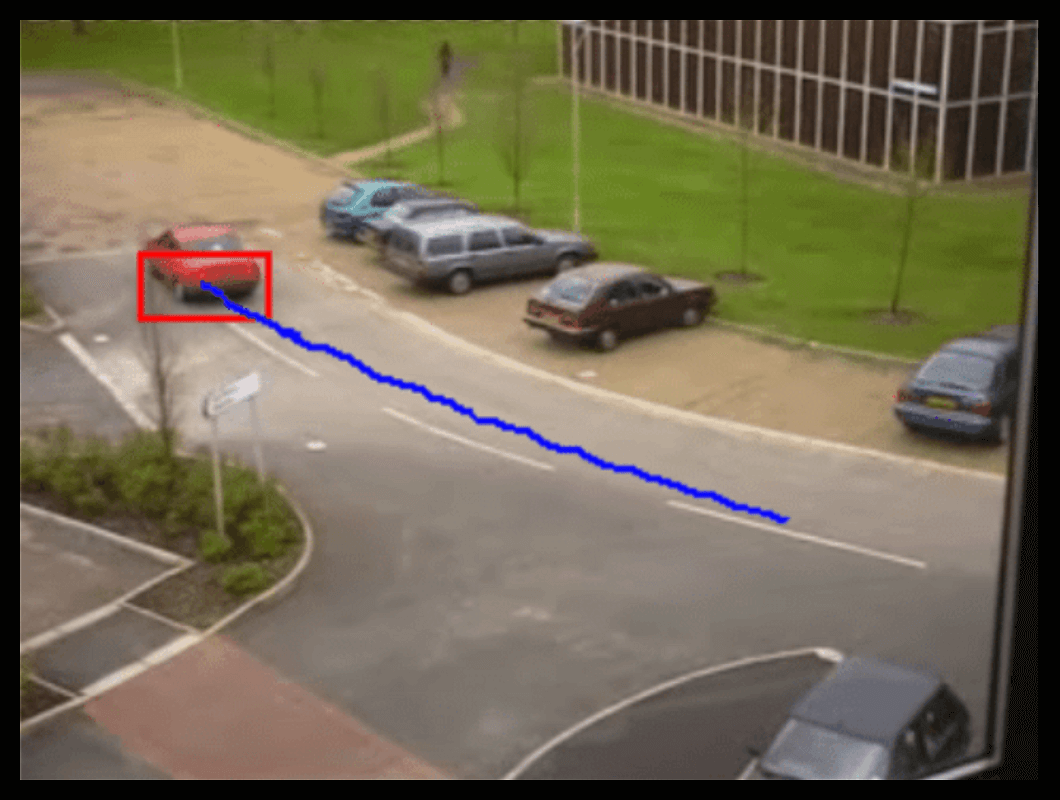
\includegraphics[width=\linewidth]{figures/chapter_tracking/sot.png}
        \caption{\acrshort{sot} }
        \label{fig:sot} 
    \end{subfigure}
    \begin{subfigure}[b]{0.61\textwidth}
        \centering
        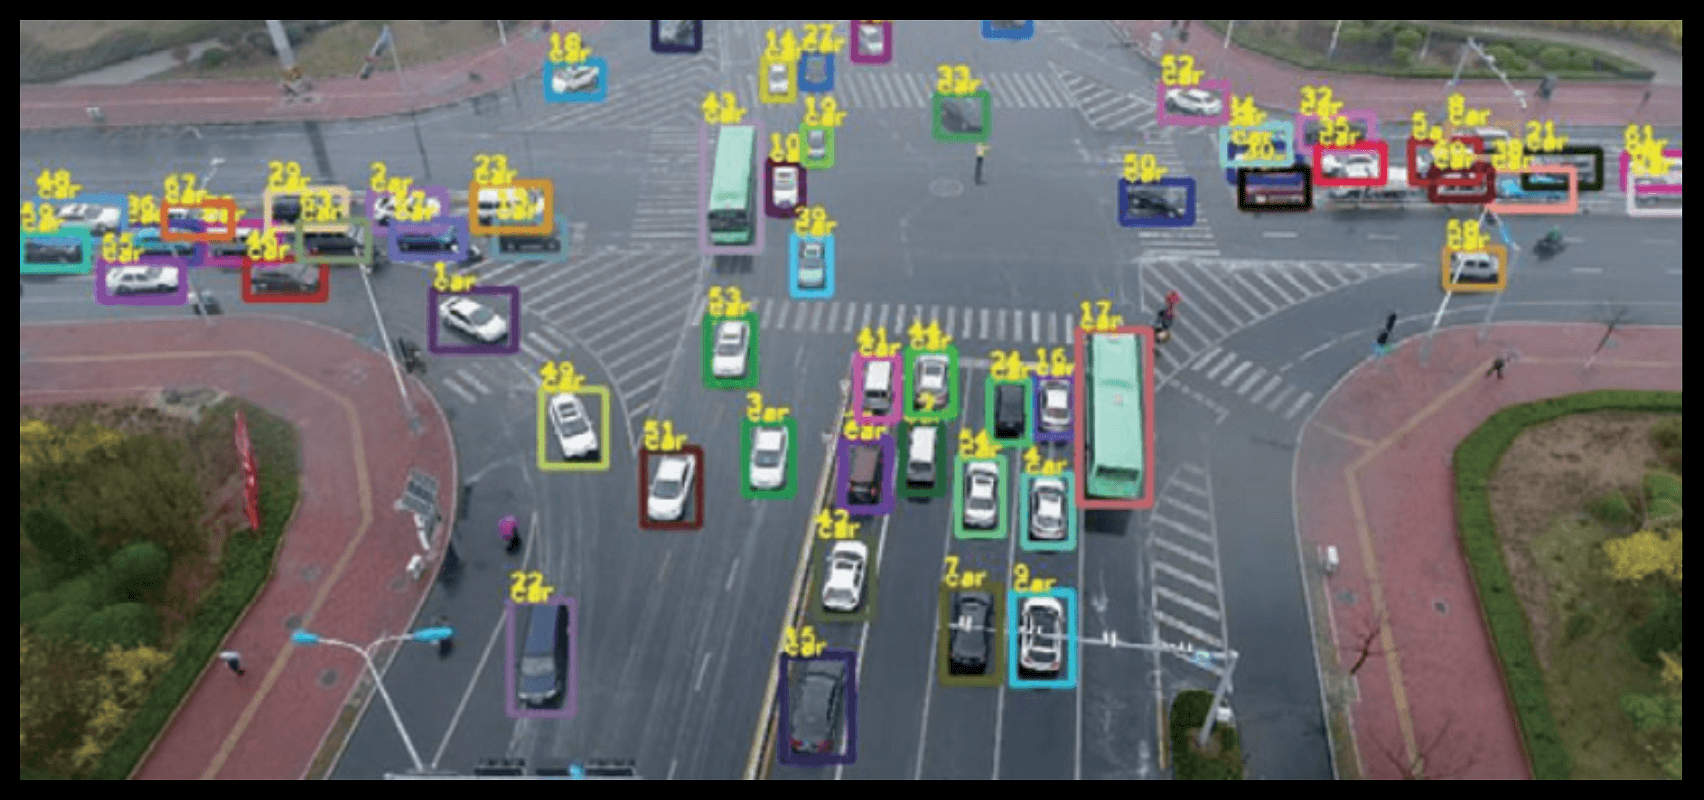
\includegraphics[width=\linewidth]{figures/chapter_tracking/mot.png}
        \caption{\acrshort{mot}}
        \label{fig:mot}
    \end{subfigure}
  \caption{The difference between \acrfull{sot} \citep{jansari2013real} and \acrfull{mot} \citep{liu2022multi}.}
  \label{fig:tracking}
\end{figure}

Recent research interests are shifting from \acrshort{sot} to \acrshort{mot}, especially in the context of autonomous driving, which demands a comprehensive perception of surrounding vehicles. Table \ref{tab.mot} highlights the top-performing methods on the KITTI multi-object tracking leaderboard for autonomous driving \citep{Geiger2012CVPR}.

\begin{table}[t]
\centering
\begin{tabular}{ lcccc } 
\hline
Method & Sensor & Type & Real-Time & HOTA    \\
\hline
BiTrack (Not publications yet) &    Lidar   &      -         & N & 82.69\% \\ 
LEGO \citep{zhang2023lego}   &    Lidar   &      -         & Y  & 80.75\% \\ 
CollabMOT \citep{ninh2024collabmot}   &    Stereo   &      \acrshort{tbd}         & N  & 80.02\% \\ 
RAM \citep{tokmakov2022object}    &    Mono  & \acrshort{jdt} & Y  & 79.53\% \\ 
PermaTrack \citep{tokmakov2021learning} & Mono  & \acrshort{jdt} & Y  & 78.03\% \\ 
\textbf{OC-SORT \citep{cao2023observation}}    & \textbf{Mono}  & \textbf{\acrshort{tbd}} & \textbf{Y}  & \textbf{76.54\%} \\ 
\hline
\end{tabular}
\caption{Top \acrfull{mot} methods on the KITTI leaderboard.}
\label{tab.mot}
\end{table}

\subsubsection{Object Tracking Sensors}

Camera and Lidar are the two most popular sensors used in autonomous vehicles. On the KITTI leaderboard, the method that utilizes point clouds from a Velodyne laser scanner achieves the highest Higher Order Tracking Accuracy (HOTA) \citep{Luiten2020IJCV}. We introduce the \acrshort{hota} evaluation metric in Sec. \ref{sec:tracking_eval}.

\textbf{Monocular Tracker}:  Vision-only methods rely solely on input images from a single camera \citep{wu2021track} \citep{hu2022monocular} are accurate for 2D multi-object tracking. However, they cannot reliably predict 3D locations because depth information is absent from single-camera input.

\textbf{Binocular Tracker}: This approach combines 2D object detection results with depth information obtained from stereo vision to achieve 3D object detection and tracking. However, using a stereo camera setup requires extensive calibration and complex matching algorithms \citep{ninh2024collabmot}.

\textbf{Multi-Modality Tracker}: Accurately estimating vehicles' pose in 3D space is crucial for autonomous driving. By combining 2D detection results with 3D Lidar data, this approach achieves the highest tracking accuracy on the KITTI leaderboard, though at the cost of using more expensive 3D laser scanners than CMOS cameras.

% \clearpage

\subsubsection{Object Tracking Frameworks}
\label{sec:tracking_framework}

\acrfull{tbd} and \acrfull{jdt} are the two most popular frameworks for object tracking applications.

\textbf{\acrfull{tbd}} is a modular object tracking framework that consists of object localization, feature extraction, data association, and track management (see Fig. \ref{fig:tbd}). Object detection models handle object localization and feature extraction to generate bounding boxes, while traditional methods such as the Hungarian Algorithm manage data association, and the Kalman Filter oversees track management. The overall accuracy of the TBD framework depends significantly on the precision of the detector, such as SiamRPN++ \citep{li2019siamrpn++} for \acrshort{sot} and YOLO, Faster R-CNN, and SSD for \acrshort{mot} applications \citep{sun2020survey}.

\textbf{\acrfull{jdt}}: As more accurate and efficient deep neural networks, such as Vision Transformer \citep{dosovitskiy2020image}, are being developed, there is also a growing trend of employing end-to-end tracking models \citep{pal2021deep, guo2022review}. PermaTrack is a \acrshort{jdt} method that takes multiple frames of images as input and outputs the position and velocity of each vehicle (see Fig. \ref{fig:jdt}). As can be seen from Tab. \ref{tab.mot}, \acrshort{jdt} methods achieve slightly higher accuracy than \acrshort{tbd} methods.

% \item Transformer: More accurate, but computationally expensive \citep{meinhardt2022trackformer} for 2D MOT \citep{lin2021swintrack}.

To explore whether traditional statistical methods, such as the Kalman Filter, can help mitigate the impact of adversarial attacks, we focus on modular \acrshort{tbd} methods (highlighted in Tab \ref{tab.mot}) instead of end-to-end \acrshort{jdt} models. Additionally, due to the lower cost and ease of setup of monocular cameras compared to 3D Lidar and stereo cameras, our primary focus is on vision-only monocular 2D object detection.

% Object Tracking Assumptions: 

% \begin{enumerate}
%     \item Camera is not moving instantly to new viewpoint.
%     \item Objects do not disappear and reappear in different places in the scene.
%     \item If the camera is moving, there is a gradual change in pose between camera and scene.
% \end{enumerate}

\begin{figure}[H]
    \centering
    \begin{subfigure}[b]{\textwidth}
        \centering
        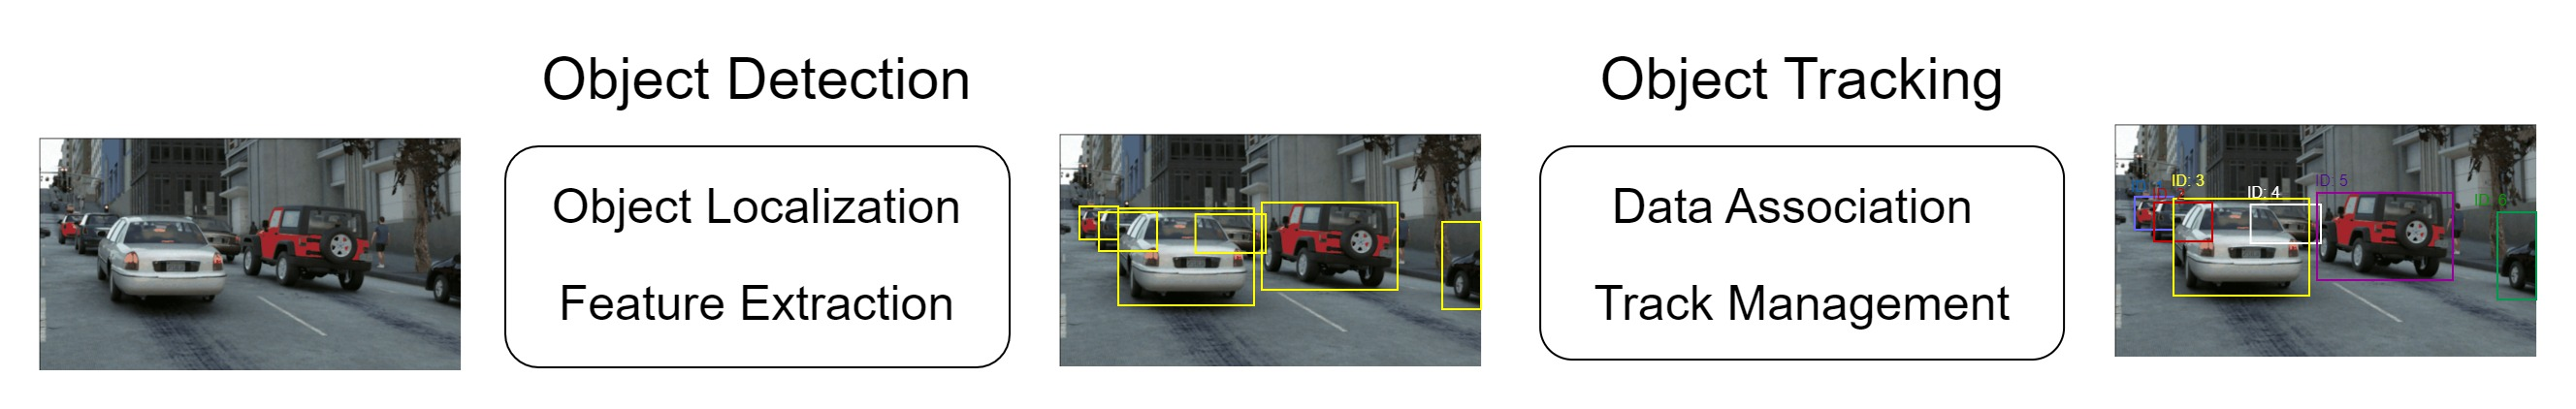
\includegraphics[width=\linewidth]{figures/chapter_tracking/tbd.jpg}
        \caption{\acrlong{tbd} (Modular System)}
        \label{fig:tbd} 
    \end{subfigure}
    \begin{subfigure}[b]{\textwidth}
        \centering
        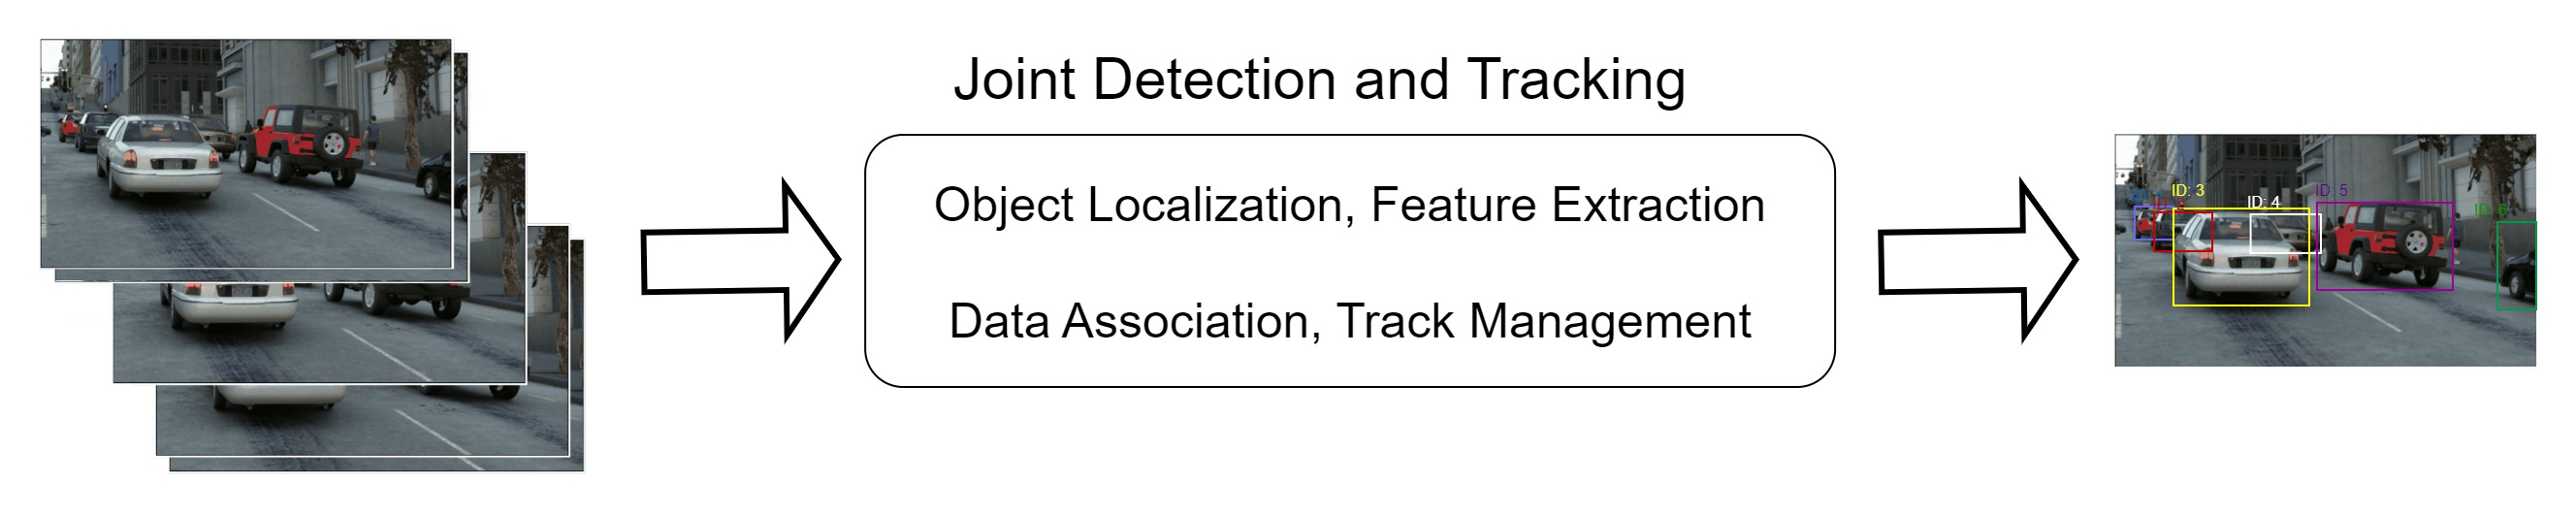
\includegraphics[width=\linewidth]{figures/chapter_tracking/jdt.jpg}
        \caption{\acrlong{jdt} (End-to-End Model)}
        \label{fig:jdt}
    \end{subfigure}
  \caption{The difference between \acrfull{tbd} and \acrfull{jdt}.}
  \label{fig:tracking_framework}
\end{figure}

% \clearpage

\subsection{Adversarial Attacks}

Adversarial attacks have progressed from image classification to object detection and then object tracking models. Notably, \acrfull{jdt} methods that utilize end-to-end deep learning models, such as GOTURN \citep{wiyatno2019physical} and FairMOT \citep{lin2021trasw}, are vulnerable to adversarial attack. For \acrfull{tbd} methods, adversaries focus on vulnerabilities in various components within the tracking system, including the object detector, the association method, and the tracklet management module.

\textbf{Attacking Object Detectors}: The accuracy of \acrshort{tbd} methods heavily relies on the object detector's ability to produce precise bounding boxes of target objects. If the object detector produces bounding boxes at incorrect positions or does not predict bounding boxes at all, the subsequent modules will struggle to generate precise tracklets. 

Table \ref{tab.mot_attack} presents studies focusing on attacking object detectors, and most work attacks SiameseRPN-based trackers  \citep{wu2019sta}. Siamese neural networks employ triplet loss or contrastive loss to train a similarity function to discern objects, such as distinguishing facial features in face recognition systems. 

In 2019, the first adversarial attack against \acrshort{mot} models attacked a \acrshort{tbd} method that used YOLOv3 as the object detector \citep{jia2020fooling}. Moreover, YOLOX \citep{ge2021yolox} and CenterNet \citep{duan2019centernet} stand out as two widely-used object detectors for autonomous driving applications, yet they both exhibit vulnerability to adversarial attacks \citep{zhou2023f,pang2024blinding}.

\textbf{Attacking Association Methods}: Another crucial factor for \acrshort{mot} system is to assign a unique ID to each detected object. It is possible to perturb the association module so that the same object may be given different IDs in different frames, thus breaking the continuity of tracklets. Liu et al. introduced the Blind Attack, which assigns the background label to the target object, and the Blur Attack, which assigns other labels to the target object \citep{liu2022efficient}.


\textbf{Attacking Tracklets}: Tracklets, commonly managed by the Kalman Filter, store the position and velocity of each vehicle. By perturbing objects' speed and direction, incorrect states are predicted for each object, enabling the switching of tracklets between adjacent objects. For instance, Lin et al. perturbed the appearance and distance similarity of two adjacent pedestrians, causing FairMOT and ByteTrack models to fail to track the targets in the subsequent frames \citep{lin2021tracklet}.

While it is acknowledged that \acrshort{mot} systems utilizing 3D Lidar Point Clouds are also susceptible to adversarial attacks \citep{cheng2021universal, cheng2022non, wang2022adversary}, our research focuses on attacks targeting vision-only \acrshort{mot} systems.

\clearpage

\begin{sidewaystable}
\centering
\begin{tabular}{ clccccc } 
\hline
Year & Method & Tracking & Model & Attack Type & Patch / Filter \\
\hline
2019 & Hijacking Attack \citep{jia2020fooling} & MOT & Yolov3 & Whitebox & Digital Patch \\
2019 & EOT Attack \citep{wiyatno2019physical} & SOT & GOTURN & Whitebox & Physical Patch \\
2020 & SPARK Attack \citep{guo2020spark} & SOT & SiamRPN++  & Whitebox & Digital Filter  \\
2020 & One-Shot Attack \citep{chen2020one} & SOT & Siamese Tracker  & Whitebox & Digital Filter \\
2020 & FAN Attack \citep{liang2020efficient} & SOT & Siamese Network & Whitebox & Digital Filter  \\
2020 & Hijacking Tracker \citep{yan2020hijacking}& SOT & SiamRPN & Whitebox & Digital Filter \\
2020 & Cool-Shrink Attack \citep{yan2020cooling} & SOT & SiamRPN++ & Whitebox & Digital Filter \\
2021 & Tracklet-Switch Attack \citep{lin2021tracklet} & MOT & FairMOT \& ByteTrack & Whitebox & Digital Filter \\
2021 & MTD Attack \citep{ding2021towards} & SOT & SiamRPN++  & Whitebox & Physical Patch \\
2021 & ABA Attack \citep{guo2021learning} & SOT & SiamRPN++ & Whitebox & Digital Blurry \\
2021 & IoU Attack \citep{jia2021iou} & SOT & SiamRPN++ & Blackbox & Digital Filter  \\
2022 & Few-Shot Attack \citep{li2022few} & SOT & SiamFC++  & Whitebox & Physical Patch\\
2022 & Ad2 Attack \citep{fu2022ad} & SOT & SiamAPN & Whitebox & Digital Filter \\
2022 & Shuffle Attack \citep{liu2022efficient} & SOT & Yolov3 + Kalman & Whitebox & Digital Filter  \\
2022 & Diminishing \citep{suttapak2022diminishing} & SOT & SiamRPN++ & Whitebox & Digital Filter    \\
2023 & F\&F Attack \citep{zhou2023f} & MOT & YOLOX \& CenterNet & Whitebox & Digital Filter  \\
2024 & Blinding \& Blurring Attack \citep{pang2024blinding} & MOT & YOLOX \& CenterNet & Whitebox & Digital Filter \\
\hline
\end{tabular}
\caption{Adversarial Attacks against Object Tracking Models.}
\label{tab.mot_attack}
\end{sidewaystable}

\clearpage

\section{Methodology}

\subsection{Problem Formulation}

For autonomous driving applications, there is no access to future frames, making it an online tracking problem, which means the model can only use past and present information to make hypothesis for the present. As introduced in Sec. \ref{sec:research_question}, we aim to answer the question: Can traditional methods mitigate the impact of adversarial attacks? To explore this, we choose the \acrshort{tbd} framework as our target model, which consists of object detection, state estimation, and data association, incorporating both deep neural networks and traditional algorithms (see Fig. \ref{fig:tracking_module}).

\vspace{0.2cm}

\noindent\textbf{Object Detection}: We use similar notations as in Chapter \ref{chpt:detection} to formulate the detection problem. To differentiate the model's hypotheses from ground truths, we use $\{h_1, h_2, h_3, ..., h_m\}$ to represent hypotheses and $\{o_1, o_2, o_3, ..., o_n\}$ as the ground truths. Given an input image $x$ at time $t$, the object detection model outputs a hypothesis of $N$ candidate bounding boxes $\{h_1^t, h_2^t, h_3^t, ..., h_N^t\}$. Each hypothesis $h_i^t=(b_i, c_i, p_i)$ includes a bounding box $b_i=(b^x_i, b^y_i, b^w_i, b^h_i)$, the confidence value $c_i \in [0, 1]$ and the softmax probability vector, $p_i=(p^1_i, p^2_i, ..., K_i)$ for $K$ classes.

\vspace{0.2cm}

\noindent\textbf{State Estimation}: To assign a consistent ID to the same object across frames, the Kalman Filter is commonly used to track the state of each object. The state of each object, modeled using a linear constant velocity model, is stored as a vector:
\begin{equation}
    \bm{x} = [u, v, s, r, \dot{u}, \dot{v}, \dot{s}]^T
\end{equation}
where $(u, v)$ are the coordinates in the image, s represents the scale, r is the aspect ratio of the object, and $[\dot{u}, \dot{v}, \dot{s}]$ are the corresponding velocities. The state vector is updated if a predicted bounding box is associated with the object.

\vspace{0.2cm}

\begin{figure}[H]
    \centering
    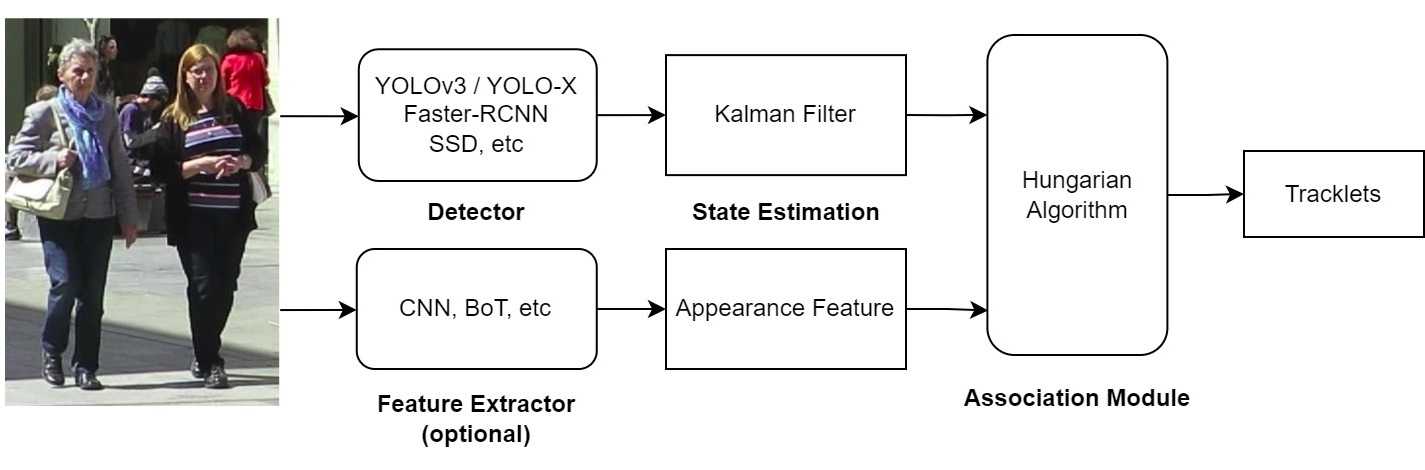
\includegraphics[width=\linewidth]{figures/chapter_tracking/track_module.jpg}
  \caption{Common modules in online tracking methods that adopt the \acrshort{tbd} framework.}
  \label{fig:tracking_module}
\end{figure}


\noindent\textbf{Feature Extractor (Optional)}: The state of each object may not be sufficient to differentiate objects when occlusion occurs. Some detection frameworks use another deep neural network, such as a Siamese Network \citep{li2019siamrpn++}, to learn a similarity function that produces a feature vector for each object and can be used to differentiate objects. However, using another deep neural network requires more computational power to achieve real-time performance, and thus, it is not utilized in all online tracking models.

\vspace{0.2cm}

\noindent\textbf{Data Association}: Besides object detection, the tracking model assigns unique IDs to each object. The association module combines the state vector and feature vector to measure the similarity between the predicted objects and ground truths. For instance, the Mahalanobis distance is often used to measure the similarity between state vectors. Then, similar objects can be associated with the same IDs by solving a linear assignment problem using the Hungarian Algorithm.

\subsection{Adversarial Tracking}

Although object detection models are vulnerable to adversarial attacks, the impact of such attacks can be mitigated if false positive bounding boxes generated by adversarial perturbations are inconsistent with the linear velocity model maintained by the Kalman Filter or cannot be associated with previous frames. In other words, the state estimation and data association methods that use traditional algorithms can filter out inconsistent bounding boxes crafted by adversarial attacks.

The accuracy of a tracking method can be easily improved with a better detection model, even if the Kalman Filter (KF) and Hungarian Algorithm remain unchanged (see Tab. \ref{tab.mot_modules}). For instance, Strong-SORT outperforms Deep-SORT partly because it adopts a more accurate detector and feature extractor that were not available when Deep-SORT was proposed. Therefore, it is crucial to use the same detection model and feature extractor across all methods for a fair comparison of state estimation and data association methods. Consequently, we use a less accurate detection model, YOLOv3, along with the same attack methods described in Chapter \ref{chpt:detection}, to test the robustness of state estimation and assignment modules.

\begin{table}[H]
\centering
\begin{tabular}{ lcc } 
\hline
Method & Detector & State Estimation \\
\hline
SORT \citep{bewley2016simple} &    FRCNN   &   KF \\
Deep-SORT \citep{wojke2017simple}  &    FRCNN   &      KF  \\ 
Strong-SORT \citep{du2023strongsort}  &    YOLOX   &      NSA KF  \\ 
OC-SORT \citep{cao2023observation} &    YOLOX  & KF \& Re-Update \\ 
\hline
\end{tabular}
\caption{A comparison of different real-time online trackers.}
\label{tab.mot_modules}
\end{table}

\clearpage

\section{Evaluation metrics}
\label{sec:tracking_eval}

Object tracking models should distinguish between different objects and consistently assign the same ID to the same object across frames. However, the IDs assigned by the tracking model do not need to match the ground truth IDs exactly. For example, a person labeled as "person 6" in the ground truth might be assigned "person 1" by the tracking model (see Fog. \ref{fig:tracking_match}). As long as the ID remains consistent across frames, the specific numbers do not need to match.

Consequently, to evaluate an object tracking model, we first need to find a one-to-one match that maps the IDs assigned by the tracking model to the IDs in the ground truths. The matching should minimize the total distance between the detected objects and their corresponding ground truth objects in all frame \citep{ciaparrone2020deep}. Finding the match can be formulated as a minimum weight assignment problem, which can be solved using the Hungarian algorithm.

\begin{figure}[H]
    \centering
    \begin{subfigure}[b]{0.48\textwidth}
        \centering
        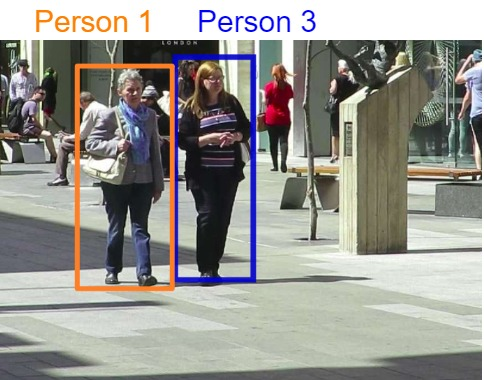
\includegraphics[width=\linewidth]{figures/chapter_tracking/eval_hypo.jpg}
        \caption{Hypotheses}
        \label{fig:track_hypo} 
    \end{subfigure}
    \begin{subfigure}[b]{0.48\textwidth}
        \centering
        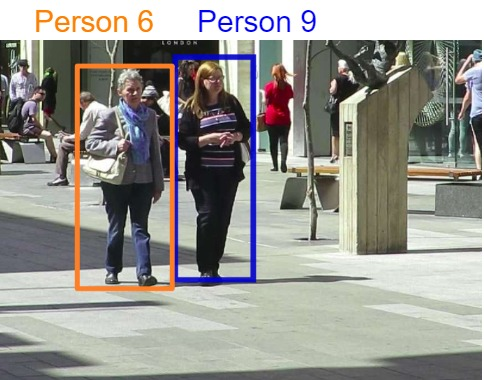
\includegraphics[width=\linewidth]{figures/chapter_tracking/eval_truth.jpg}
        \caption{Ground Truths}
        \label{fig:track_true}
    \end{subfigure}
  \caption{The same person may be assigned a different ID by the tracking model compared to the ground truth.}
  \label{fig:tracking_match}
\end{figure}

After finding the match, the tracking results can be evaluated using the following widely adopted evaluation metrics MT, ML \citep{wu2006tracking}, MOTA \citep{bernardin2008evaluating}, IDF1 \citep{ristani2016performance}, and HOTA \citep{luiten2021hota}.

\subsection{Classical Metrics (MT, ML)}

\acrfull{mt} and \acrfull{ml} are the two most popular evaluation metrics proposed in \citep{wu2006tracking} and are widely reported in MOTChallenge \citep{dendorfer2020mot20}, KITTI \citep{Geiger2012CVPR} and nuScenes \citep{caesar2020nuscenes} dataset.

For the video frame at time $t$, the object tracking model assigns a unique ID $j$ to a detected object and produces a hypothesis $h_j^t$. After solving the linear assignment problem using the Hungarian Algorithm, if the hypothesis $h_j^t$ is mapped to $o_i^t$ (see \ref{fig:mt_ml}), the ground truth object is considered tracked at time step t.

Ground truth objects with the same ID at different time steps are combined into a tracklet. A tracklet is classified as mostly tracked if correctly tracked in at least 80\% of the frames. Conversely, a tracklet is classified as mostly lost if correctly tracked in at most 20\% of the frames. The evaluation metric \acrshort{mt} counts the number of mostly tracked tracklets, while \acrshort{ml} counts the number of mostly lost tracklets.

\begin{figure}[H]
    \centering
    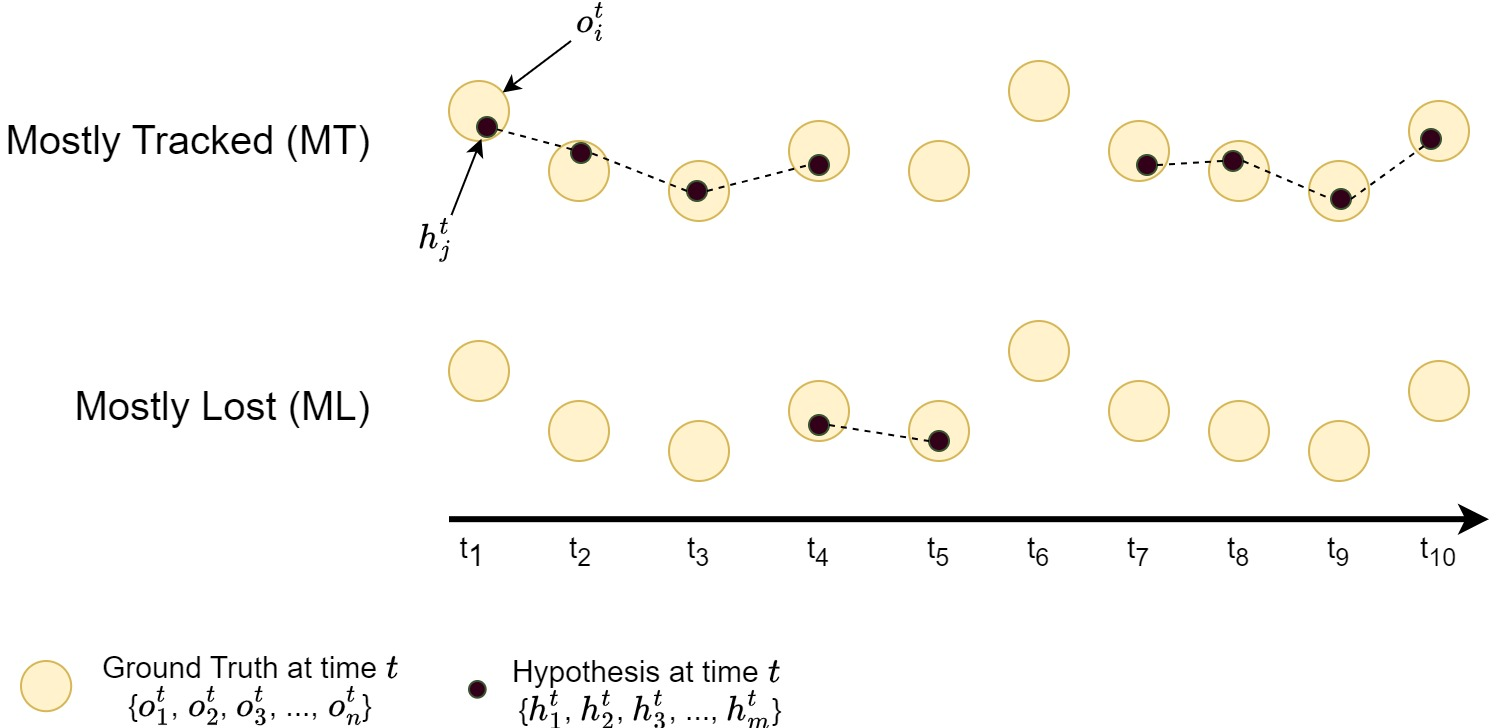
\includegraphics[width=\linewidth]{figures/chapter_tracking/MT_ML.jpg}
  \caption{Examples of mostly tracked and mostly lost tracklets.}
  \label{fig:mt_ml}
\end{figure}


\subsection{CLEAR MOT Metrics (MOTA)}

Although MT and ML count the total number of good (mostly tracked) tracklets and bad (mostly lost) tracklets, they do not provide information about the bottleneck of the tracker or how to improve it. These metrics do not indicate whether improvements should be focused on the detector or the association algorithm.

To address this issue, the CLEAR MOT Metrics use the number of False Positives and False Negatives to measure the accuracy of the detector, and ID Switches to measure the quality of the association algorithm. An overall metric, MOTA, is then calculated to provide a comprehensive evaluation.

\begin{equation}
    MOTA = 1 - \frac{ \sum_t FN_t + \sum_t FP_t + \sum_t IDSW_t}{\sum_t GT_t} \in (-\infty, 1] 
\end{equation}

As illustrated in Fig. \ref{fig:track_mota_fp_fn}, the tracking result is accurate if a ground truth is matched with a hypothesis. A false negative (FN) is counted when a ground truth bounding box cannot be associated with a hypothesis (the left side), and a false positive (FP) is counted when a hypothesis cannot be associated with a ground truth bounding box (the right side). Besides, the ID switch happens when the same ground truth object is assigned different IDs in consecutive frames (see Fig. \ref{fig:track_mota_idsw}).

\begin{figure}[H]
    \centering
    \begin{subfigure}[b]{\textwidth}
        \centering
        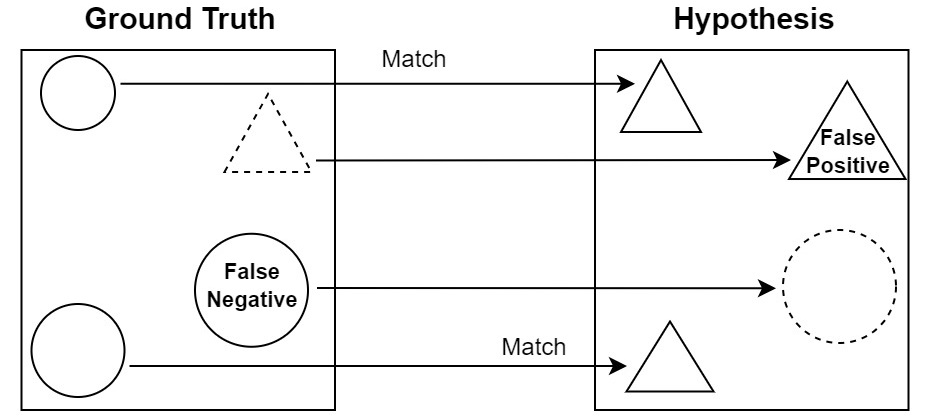
\includegraphics[width=\linewidth]{figures/chapter_tracking/MOTA_FP_FN.jpg}
        \caption{False Negative and False Positive.}
        \label{fig:track_mota_fp_fn} 
    \end{subfigure}
    \begin{subfigure}[b]{\textwidth}
        \centering
        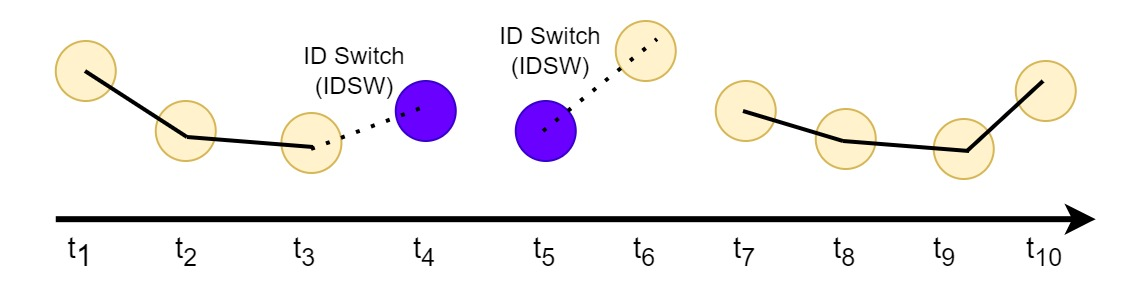
\includegraphics[width=\linewidth]{figures/chapter_tracking/MOTA_IDSW.jpg}
        \caption{ID Switch}
        \label{fig:track_mota_idsw}
    \end{subfigure}
  \caption{The False Negatives (FN), False Positives (FP) and ID Switches (IDSW) for \acrfull{mota}.}
  \label{fig:tracking_mota}
\end{figure}

\subsection{ID Scores (IDF1)}

While the MOTA provides information about how the detector performs using FN and FP, and use IDSW to evaluate association algorithm, it is biased towards detection. For instance,

\begin{figure}[H]
    \centering
    \begin{subfigure}[b]{\textwidth}
        \centering
        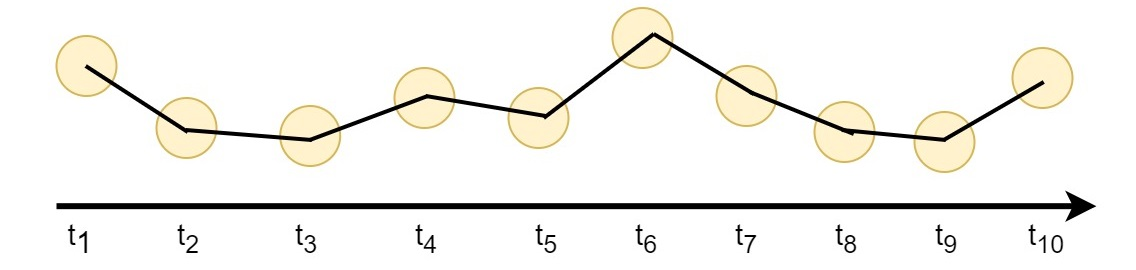
\includegraphics[width=\linewidth]{figures/chapter_tracking/IDSW_gt.jpg}
        \caption{The ground truth tracklet.}
        \label{fig:track_idf1_gt} 
    \end{subfigure}
    \begin{subfigure}[b]{\textwidth}
        \centering
        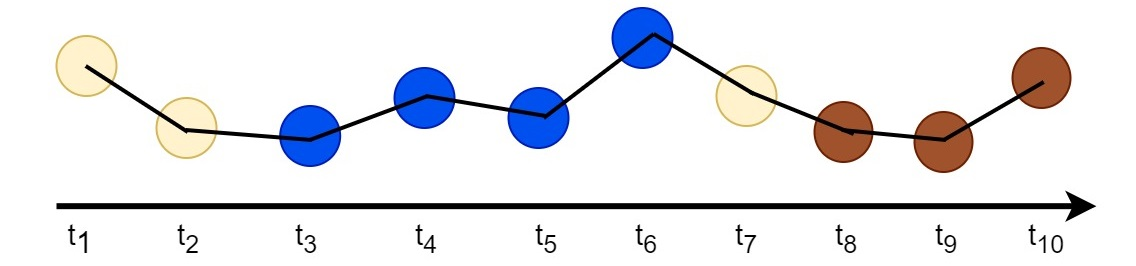
\includegraphics[width=\linewidth]{figures/chapter_tracking/IDSW_track_1.jpg}
        \caption{Tracklet 1: \textbf{MOTA = 70\%} (FN=0, FP=0, IDSW=3), \textbf{IDF1 = 30\%} (IDTP = 3, IDFP = 7, IDFN = 7) }
        \label{fig:track_idf1_track_1}
    \end{subfigure}
    \begin{subfigure}[b]{\textwidth}
        \centering
        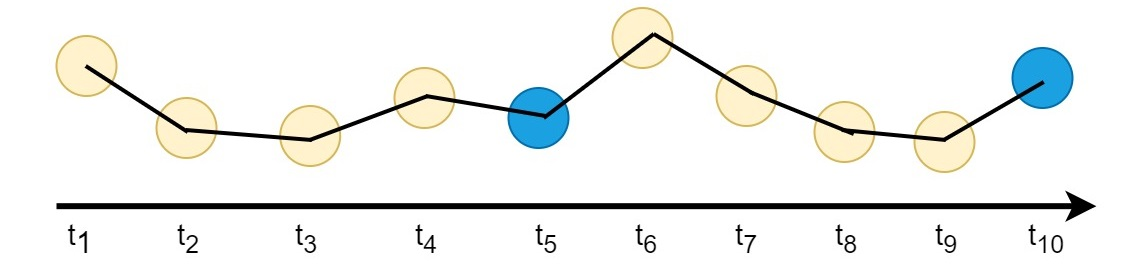
\includegraphics[width=\linewidth]{figures/chapter_tracking/IDSW_track_2.jpg}
        \caption{Tracklet 2: \textbf{MOTA = 70\%} ((FN=0, FP=0, IDSW=3), \textbf{IDF1 = 80\%} (IDTP = 8, IDFP = 2, IDFN = 2)}
        \label{fig:track_idf1_track_2}
    \end{subfigure}
  \caption{A comparison of MOTA and IDF1. Different colors indicate different IDs assigned by the tracking model.}
  \label{fig:tracking_idf1}
\end{figure}

To address these issues, we propose to measure performance not by how often mismatches occur, but by how long the tracker correctly identifies targets.

Bipartite graphs are commonly used to model matching problems,

\begin{figure}[H]
    \centering
    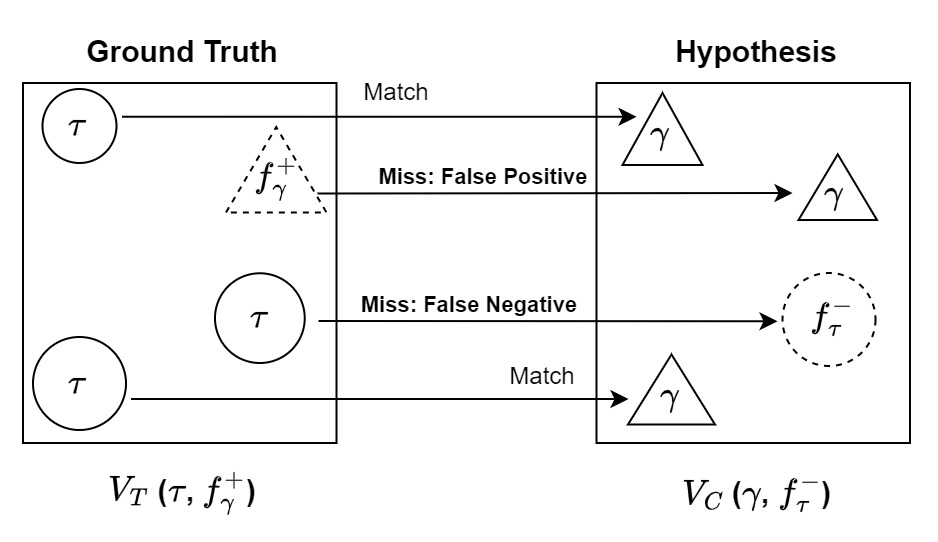
\includegraphics[width=\linewidth]{figures/chapter_tracking/bipartite.jpg}
  \caption{Bipartite Graph for IDF1 score.}
  \label{fig:idf1_bipartite}
\end{figure}

To this end, ground-truth identities are first matched to computed ones.

\begin{equation}
    \text{IDP} = \frac{\text{IDTP}}{\text{IDTP} + \text{IDFP}} \quad 
    \text{IDR} = \frac{\text{IDTP}}{\text{IDTP} + \text{IDFN}}
\end{equation}

\begin{equation}
    \text{IDF}_1 = \frac{2 \text{IDTP}}{2 \text{IDTP} + \text{IDFP} + \text{IDFN}}
\end{equation}

\subsection{Higher Order Tracking Accuracy (HOTA)}

The MOTA is biased towards detection, while IDF1 is biased towards association. The HOTA tries to find a balance between detection and association.

\begin{equation}
    \text{DetA}_{\alpha} = \frac{|\text{TP}_{\alpha}|}{|\text{TP}_\alpha| + |\text{FN}_\alpha| + |\text{FP}_\alpha|},
    \text{AssA}_{\alpha} = \frac{1}{|\text{TP}_\alpha|} \sum_{c \in \text{TP}} \text{Ass-IoU}(c)
\end{equation}

Then HOTA

\begin{equation}
    \text{HOTA}_{\alpha} = \sqrt{\text{DetA}_{\alpha} \cdot \text{AssA}_{\alpha}} = \sqrt{\frac{\sum_{c \in \text{TP}} \text{Ass-IoU}(c)}{|\text{TP}_{\alpha}| + | FN_{\alpha}| + | \text{FP}_{\alpha}| }}
\end{equation}

Lastly,

\begin{equation}
    \text{HOTA} = \int_{0 < \alpha \leq 1} \text{HOTA}_{\alpha} \approx \frac{1}{19} \sum_{\substack{\alpha=0.05 \\ \alpha+= 0.05}}^{0.95} \text{HOTA}_{\alpha}
\end{equation}

% \clearpage

\section{Experimental Results}

We first demonstrate the importance of detector.


\subsection{Image-Specific}


\clearpage

\subsection{Image-Agnostic}

\clearpage

\section{Summary}

% In summary, we find several research papers that attack 2D SOT (caemera) and 3D MOT ( Lidar). But we do not find attacks against 3D monocular trackers \citep{wu2021track} \citep{hu2022monocular}. Neither do we find research that attacks Transformers for 2D MOT.

% We plan to attack 3D MOT models for Vision-Based vehicle tracking in real time (no 3D Lidar Data). First, we'll implement two 3D MOT models: \href{https://github.com/SysCV/qd-3dt}{QD-3DT} and \href{https://github.com/JialianW/TraDeS}{TraDeS}. Then, we'll try to design white-box attacks to fabricate, vanish 3D bounding boxes, change their orientations, or dissociate them with actual objects.

% \clearpage

% \printbibliography[
%   keyword={chapter_tracking}, heading=subbibintoc, resetnumbers=true
% ]